
\section{Creating a Gaussian process}\label{sub:inst}

This section demonstrates creation of a covariance function, a mean function, and finally several random functions drawn from the Gaussian process distribution defined by those objects.

\subsection{Creating a mean function}\label{subsub:mean}

\begin{figure}
    \centering
        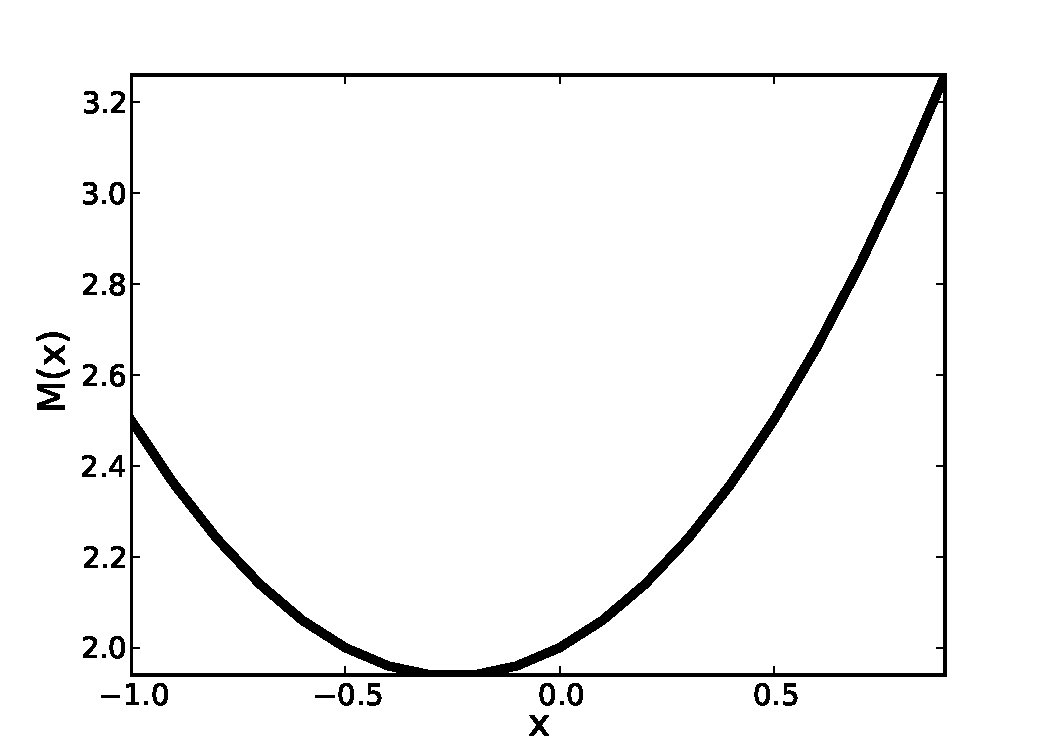
\epsfig{file=figs/mean.pdf,width=8cm}
    \caption{The mean function generated by {\sffamily `examples/mean.py'}.}
    \label{fig:mean}
\end{figure}

The mean function of a univariate Gaussian process can be interpreted as a prior guess for the GP, so it is also a univariate function. Mean functions are represented by class \code{Mean}, which is a wrapper for an ordinary \proglang{Python} function. The following code (from \code{pymc/examples/gp/Mean.py}) will produce an instance of class \code{Mean} called $M$:
\begin{CodeChunk}
\begin{CodeInput}
from pymc.gp import *
def quadfun(x, a, b, c):
    return (a * x ** 2 + b * x + c)
M = Mean(quadfun, a = 1., b = .5, c = 2.)        
\end{CodeInput}
\end{CodeChunk}

The first argument of \code{Mean}'s init method is the underlying \proglang{Python} function, in this case \code{quadfun}. The extra arguments $a$, $b$  and $c$ will be memorized and passed to \code{quadfun} whenever $M$ is called; the call $M(x)$ in the plotting portion of the script does not need to pass them in.

Mean functions broadcast over their arguments in the same way as \href{http://docs.scipy.org/doc/numpy/reference/ufuncs.html}{\pkg{NumPy} universal functions} \citep{numpybook}, which means that the call $M(x)$, where $x$ is a vector, returns the vector
\begin{eqnarray*}
    [M(x_0),\ldots, M(x_{N-1})].
\end{eqnarray*}

The last part of the code plots $M(x)$ on $-1<x<1$, and its output is shown in figure \ref{fig:mean}. As expected, the plot is a parabola.

\subsection{Creating a covariance function}\label{subsub:cov}
\begin{figure}
    \centering
        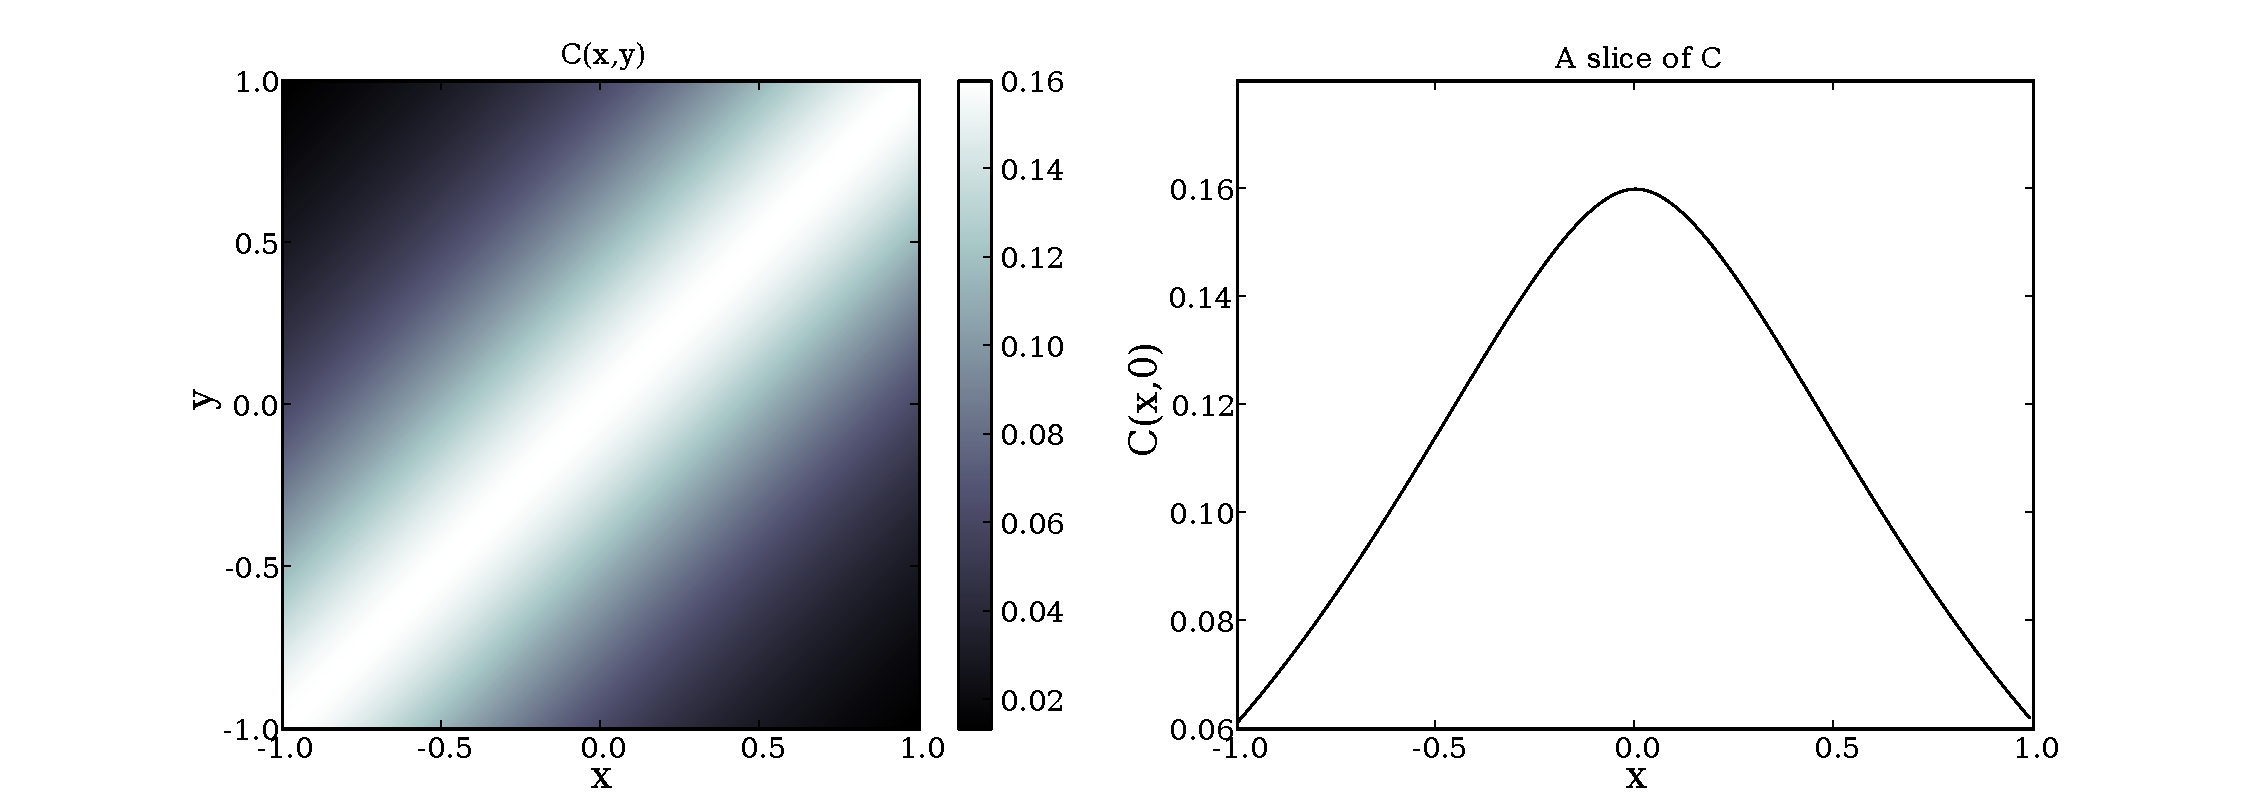
\epsfig{file=figs/cov.pdf,width=12cm}
    \caption{The covariance function generated by {\sffamily `examples/cov.py'}. On the left is the covariance function $C(x,y)$ evaluated over a square: $-1\le x\le 1,\ -1\le y\le 1$. On the right is a slice of the covariance: $C(x,0)$ for $0\le x \le 1$}
    \label{fig:cov}
\end{figure}

Covariance functions are represented by the class \code{Covariance}, which like \code{Mean} is essentially a wrapper for ordinary \proglang{Python} functions. The example in \code{pymc/examples/gp/cov.py} uses the popular Mat\`ern function \citep{banerjee}, which is provided in module \code{cov_funs}. In addition to the two arguments $x$ and $y$, the Mat\`ern function takes three parameters: \code{amp} controls the amount by which realizations may deviate from their mean, \code{diff_degree} controls the roughness of realizations (the degree of differentiability), and \code{scale} controls the lengthscale over which realizations change.

The user is free to write functions to wrap in \code{Covariance} objects. See \href{http://code.google.com/p/pymc}{the package documentation} for more information.

The code in \code{pymc/examples/gp/cov.py} will produce an instance of class \code{Covariance} called $C$:
\begin{CodeChunk}
\begin{CodeInput}
from pymc.gp import *
from pymc.gp.cov_funs import matern

C = Covariance(eval_fun = matern.euclidean, diff_degree = 1.4, amp = .4, scale = 1.)
\end{CodeInput}
\end{CodeChunk}

The first argument to \code{Covariance}'s init method is the \proglang{Python} function from which the covariance function will be made. In this case, \code{eval_fun} is \code{matern.euclidean}. Covariance functions' calling conventions are slightly different from ordinary \pkg{NumPy} universal functions' \citep{numpybook} in two ways. First, broadcasting works differently. If $C$ were a \pkg{NumPy} universal function, $C(x,y)$ would return the following array:
    \begin{eqnarray*}
        \begin{array}{ccc}
            [C(x_0,y_0)& \ldots& C(x_{N-1},y_{N-1})],
        \end{array}
    \end{eqnarray*}
    where $x$ and $y$ would need to be vectors of the same length. In fact $C(x,y)$ returns a matrix:
    \begin{eqnarray*}
        \left[\begin{array}{ccc}
            C(x_0,y_0)& \ldots& C(x_0,y_{N_y-1})\\
            \vdots&\ddots&\vdots\\
            C(x_{N_x-1},y_0)& \ldots& C(x_{N_x-1},y_{N_y-1})
        \end{array}\right],
    \end{eqnarray*}
    and input arguments $x$ and $y$ don't need to be the same length. Second, covariance functions can be called with just one argument. $C(x)$ returns
    \begin{eqnarray*}
         [C(x_0,x_0)& \ldots& C(x_{N_x-1},x_{N_x-1})] = \textup{diag}(C(x,x)),
    \end{eqnarray*}
    but is computed much faster than diag$(C(x,x))$ would be.
The extra arguments \code{diff_degree, amp} and \code{scale}, which are required by \code{matern.euclidean}, will be passed to \code{matern.euclidean} by $C$ every time is called.
 
The output of \code{examples/cov.py} is shown in figure \ref{fig:cov}.

\subsubsection{Cholesky algorithms}

The numerical `heavy lifting' done by this package is primarily handled by \code{Covariance} and its subclasses. \texttt{Covariance} itself bases all its computations on the incomplete Cholesky decomposition algorithm used by the \proglang{Matlab} package \pkg{chol_incomplete} \citep{seeger}. \code{Covariance} computes rows of covariance matrices as they are needed, so if the function it wraps tends to produce covariance matrices with only a few large eigenvalues it can approximate the Cholesky decomposition in less than $O(n^2)$ arithmetic operations \citep{predictivechol}.

\code{Covariance} calls back to \proglang{Python} from \proglang{Fortran} every time it needs a new row. If the function it wraps tends to produce full-rank covariance matrices (for which all rows are required), this is inefficient. \code{FullRankCovariance} is a drop-in replacement for \code{Covariance} that is much faster, but fails (with a helpful error message) if it attempts to factor a matrix that is not full rank. \code{NearlyFullRankCovariance} provides a compromise between the two: it computes covariance matrices in full in \proglang{Fortran}, then factors them using the robust algorithm of \pkg{chol_incomplete}.

\subsection{Drawing realizations}\label{subsub:realizations}
\begin{figure}
    \centering
        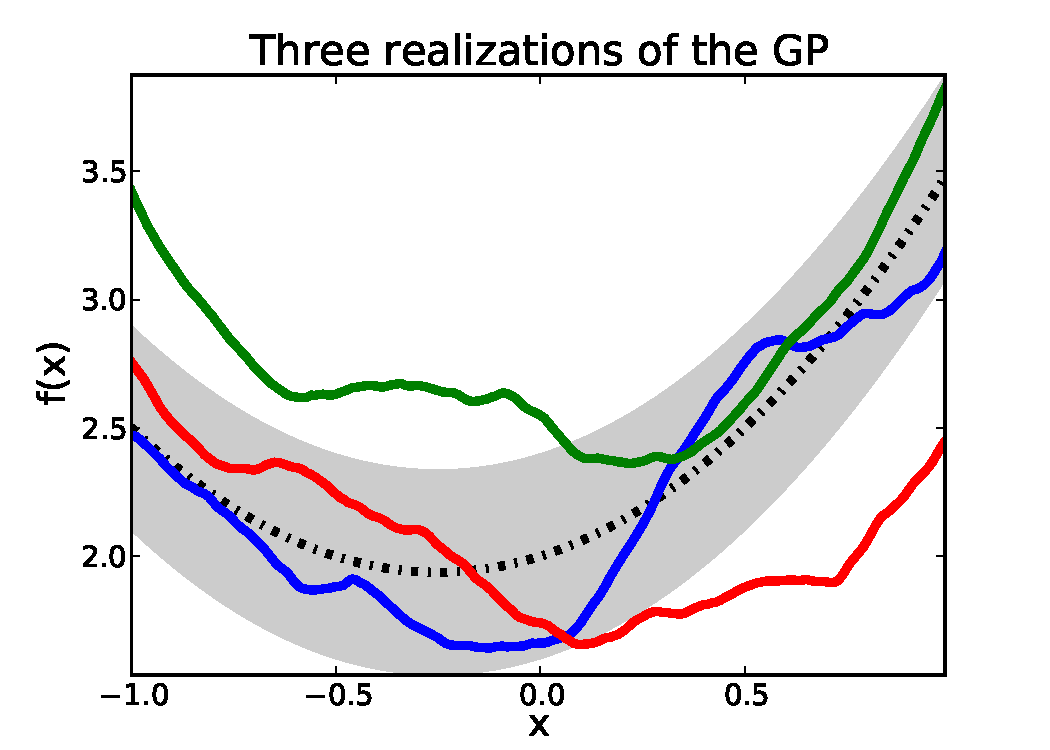
\epsfig{file=figs/realizations.pdf,width=8cm}
    \caption{Three realizations from a Gaussian process displayed with mean $\pm$ 1 sd envelope. Generated by {\sffamily `examples/realizations.py'}.}
    \label{fig:realizations}
\end{figure}

The code in \texttt{pymc/examples/gp/realizations.py} generates a list of \code{Realization} objects, which represent realizations (draws) from the Gaussian process defined by $M$ and $C$:
\begin{CodeChunk}
\begin{CodeInput}
from mean import M
from cov import C
from pymc.gp import *

f_list = [Realization(M,C) for i in range(3)]
\end{CodeInput}
\end{CodeChunk}

The init method of \code{Realization} takes only two required arguments, a \code{Mean} object and a \code{Covariance} object. Each element of \code{f_list} is a Gaussian process realization, which is essentially a randomly-generated \proglang{Python} function. Like \code{Mean} objects, \code{Realization} objects use the same broadcasting rules as \pkg{NumPy} universal functions. The call $f(x)$ returns the vector
\begin{eqnarray*}
    [f(x_0)\ldots f(x_{N-1})].
\end{eqnarray*}

Each of the three realizations in \code{f_list} is plotted in figure \ref{fig:realizations}, superimposed on a $\pm$ 1 standard deviation envelope.


\section{Nonparametric regression: observing Gaussian processes}\label{sec:observing}

\begin{figure}
    \centering
        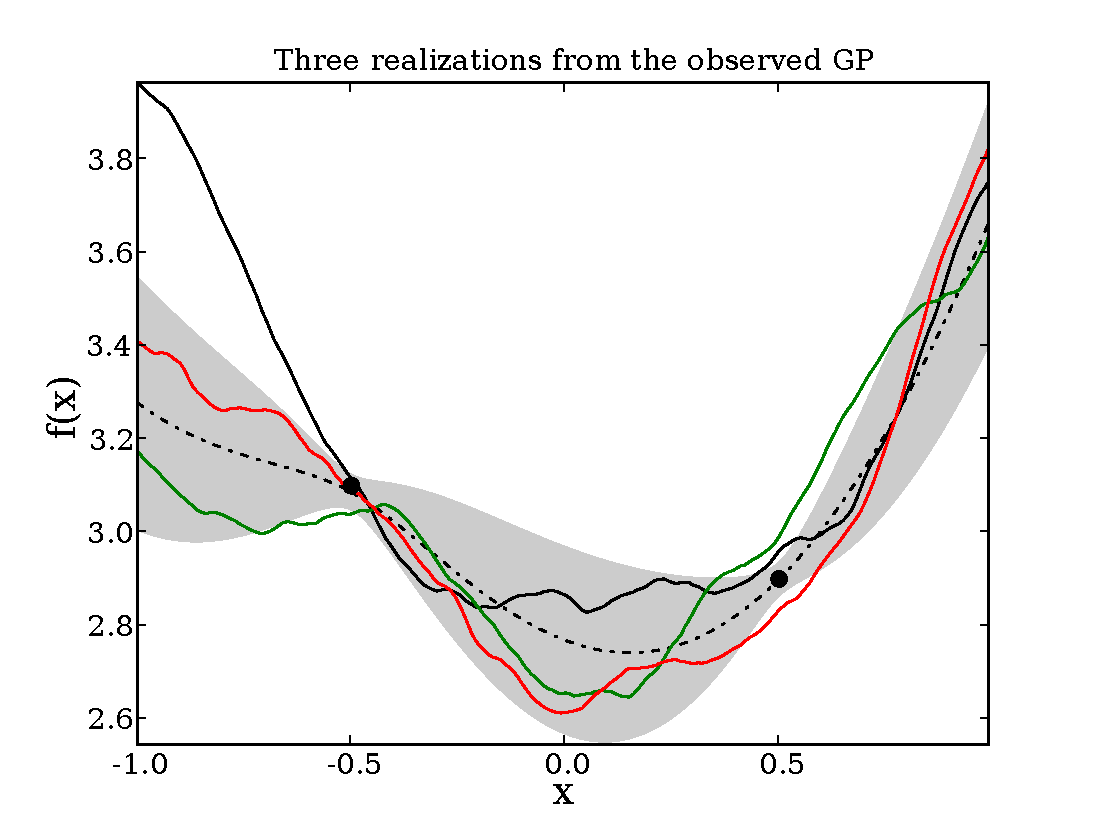
\epsfig{file=figs/obs.pdf,width=5cm}
        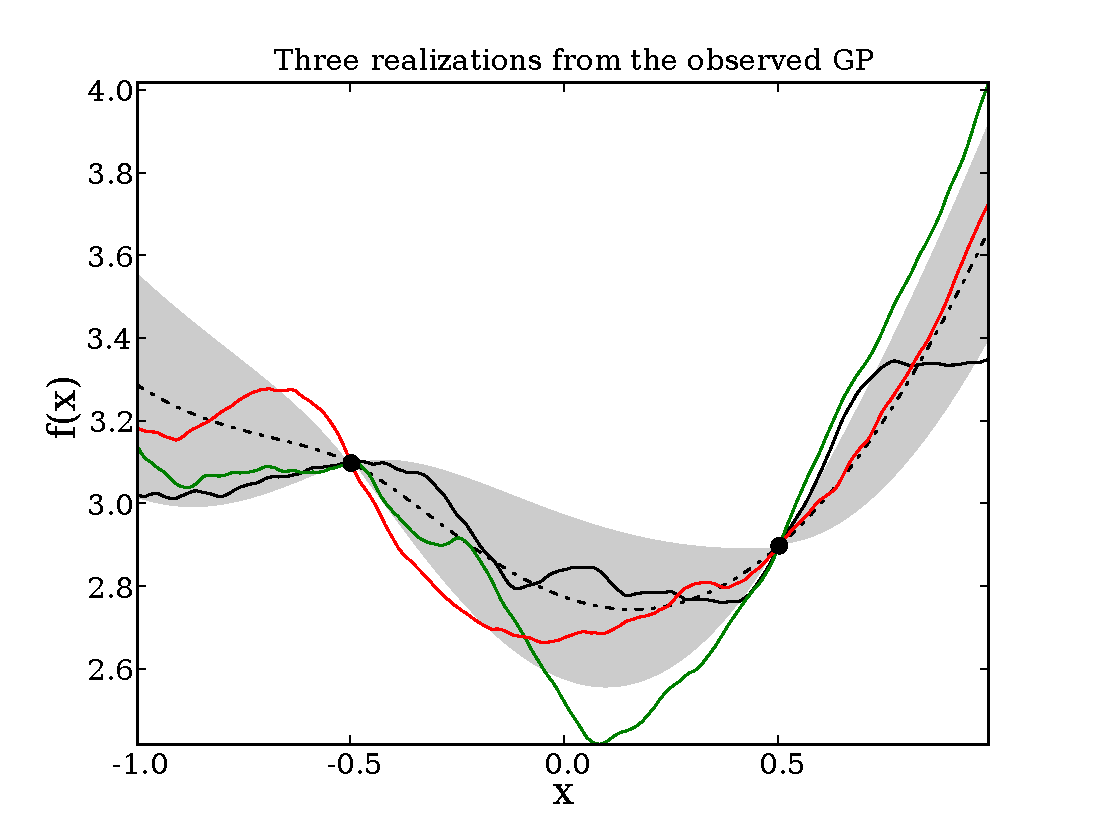
\epsfig{file=figs/cond.pdf,width=5cm}
    \caption{The output of {\sffamily `examples/observations.py'}: the observed GP with \code{obs_V = .002} (left) and \code{obs_V = 0} (right). Note that in the conditioned case, the $\pm$ 1 SD envelope shrinks to zero at the points where the observations were made, and all realizations pass through the observed values. Compare these plots to those in figure \ref{fig:realizations}.}
    \label{fig:obs}
\end{figure}

Consider the following common statistical situation: A Gaussian process prior for an unknown function $f$ is chosen, then the value of $f$ is observed at $N$ input points $[o_0\ldots o_{N-1}]$, possibly with uncertainty. If the observation error is normally distributed, it turns out that $f$'s posterior distribution given the new information is another Gaussian process, with new mean and covariance functions.

The probability model that represents this situation is as follows:
\begin{equation}
    \label{regprior}
    \left.\begin{array}{l}
        \textup{data}_i \stackrel{\tiny{\textup{ind}}}{\sim} \textup{N}(f(o_i), V_i)\\
        f \sim \textup{GP}(M,C)\\
    \end{array}\right\}\Rightarrow f|\textup{data} \sim \textup{GP}(M_o, C_o).
\end{equation}
Function \code{observe} imposes normally-distributed observations on Gaussian process distributions. This function converts $f$'s prior to its posterior by transforming $M$ and $C$ in equation \ref{regprior} to $M_o$ and $C_o$:

The code in \code{pymc/examples/gp/observation.py} imposes the observations
\begin{eqnarray*}
    f(-.5) = 3.1\\
    f(.5) = 2.9
\end{eqnarray*}
with observation variance $V=.002$ on the GP distribution defined in \code{mean.py} and \code{cov.py}:
\begin{CodeChunk}
\begin{CodeInput}
from mean import M
from cov import C
from pymc.gp import *
from numpy import *

obs_x = array([-.5,.5])
V = array([.002,.002])
data = array([3.1, 2.9])
observe(M=M, C=C, obs_mesh=obs_x, obs_V=V, obs_vals=data)

f_list = [Realization(M,C) for i in range(3)]
\end{CodeInput}
\end{CodeChunk}

The function \code{observe} takes a covariance $C$ and a mean $M$ as arguments, and tells them that their `true' realization's value on \code{obs_mesh} has been observed to be \code{obs_vals} with variance \code{obs_V}. 

The output of \code{observation.py}  is shown in figure \ref{fig:obs}, along with the output with \code{obs_V=0}. Compare these to the analogous figure for the unobserved GP, figure \ref{fig:realizations}. The covariance after observation is visualized in figure \ref{fig:obscov}. The covariance `tent' has been pressed down at points where $x\approx \pm .5$ and/or $y\approx\pm .5$, which are the values where the observations were made.

\begin{figure}
    \centering
        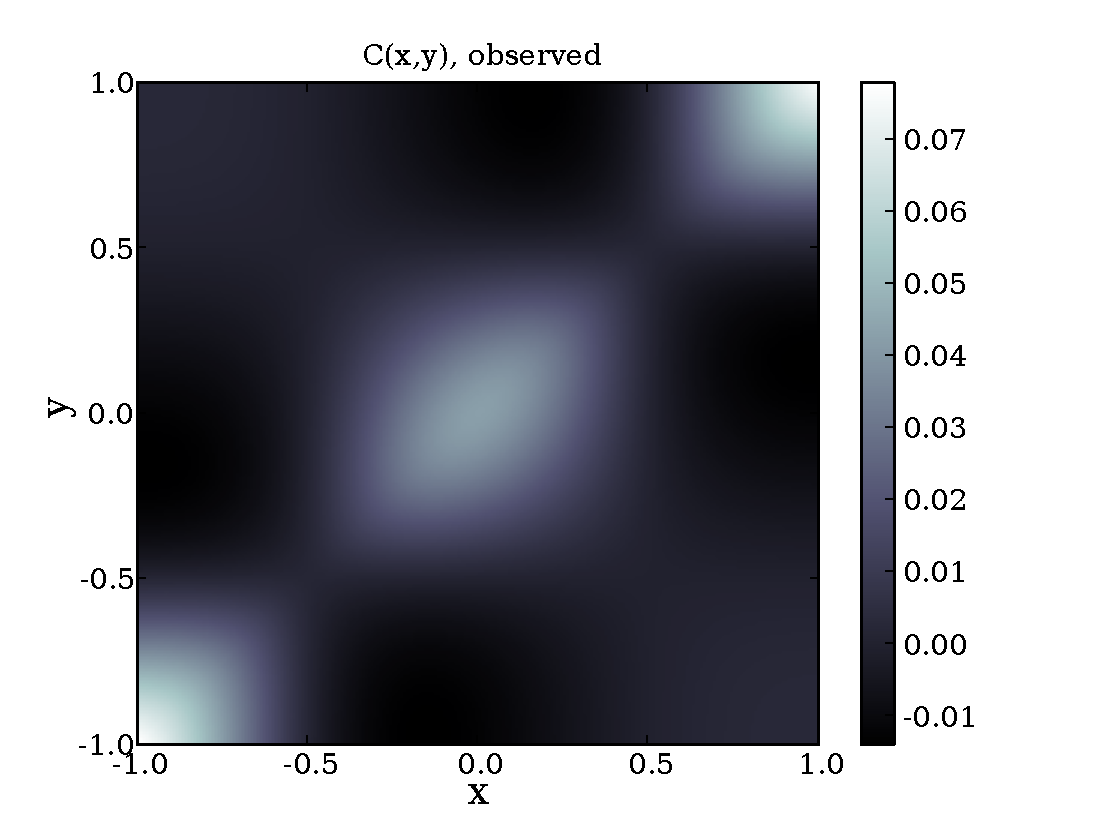
\epsfig{file=figs/obscov.pdf,width=5cm}
    \caption{The covariance function from {\sffamily `observation.py'} after observation. Compare this with the covariance function before observation, visualized in figure \ref{fig:cov} }
    \label{fig:obscov}
\end{figure}

\section{Higher-dimensional GPs}\label{sec:highdim}

In addition to functions of one variable such as $f(x)$, this package supports Gaussian process priors for functions of many variables such as $f(\mathbf{x})$, where $\mathbf{x}=[x_0\ldots x_{n-1}]$. This is useful for modeling dynamical or biological functions of many variables as well as for spatial statistics.

When array is passed into a \code{Mean}, \code{Covariance} or \code{Realization}'s init method or one of these objects is evaluated on an array, the array's last index is understood to iterate over spatial dimension. To evaluate a covariance $C$ on the ordered pairs $(0,1)$, $(2,3)$, $(4,5)$ and $(6,7)$, the user could pass in the following two-dimensional \pkg{NumPy} array:
\begin{verbatim}
[[0,1]
 [2,3]
 [4,5]
 [6,7]]
\end{verbatim}
or the following three-dimensional array:
\begin{verbatim}
[[[0,1]
  [2,3]],

  [4,5]
  [6,7]]]
\end{verbatim}
Either is fine, since in both the last index iterates over elements of the ordered pairs.

The exception to this rule is one-dimensional input arrays. The array
\begin{verbatim}
[0, 1, 2, 3, 4, 5, 6, 7]
\end{verbatim}
is interpreted as an array of eight one-dimensional values, whereas the array
\begin{verbatim}
[[0, 1, 2, 3, 4, 5, 6, 7]]
\end{verbatim}
is interpreted as a single eight-dimensional value according to the convention above.

Means and covariances learn their spatial dimension the first time they are called or observed. Some covariances, such as those specified in geographic coordinates, have an intrinsic spatial dimension. Realizations inherit their spatial dimension from their means and covariances when possible, otherwise they infer it the first time they are called. If one of these objects is subsequently called with an input of a different dimension, it raises an error.

\subsection{Covariance function bundles and coordinate systems}
The examples so far, starting with \code{examples/cov.py}, have used the covariance function \code{matern.euclidean}. This function is an attribute of the \code{matern} object, which is an instance of class \code{covariance_function_bundle}.

Instances of \code{covariance_function_bundle} have three attributes, \code{euclidean}, \code{geo_deg} and \code{geo_rad}, which correspond to standard coordinate systems:
\begin{itemize}
    \item \code{euclidean}: $n$-dimensional Euclidean coordinates.
    \item \code{geo_deg}: Geographic coordinates (longitude, latitude) in degrees, with unit radius.
    \item \code{geo_rad}: Geographic coordinates (longitude, latitude) in radians, with unit radius.
\end{itemize}

See \href{http://code.google.com/p/pymc}{the package documentation} for information regarding creation and extension of covariance function bundles.

\section{Basis covariances}\label{sec:basis}

\begin{figure}[htbp]
    \centering
        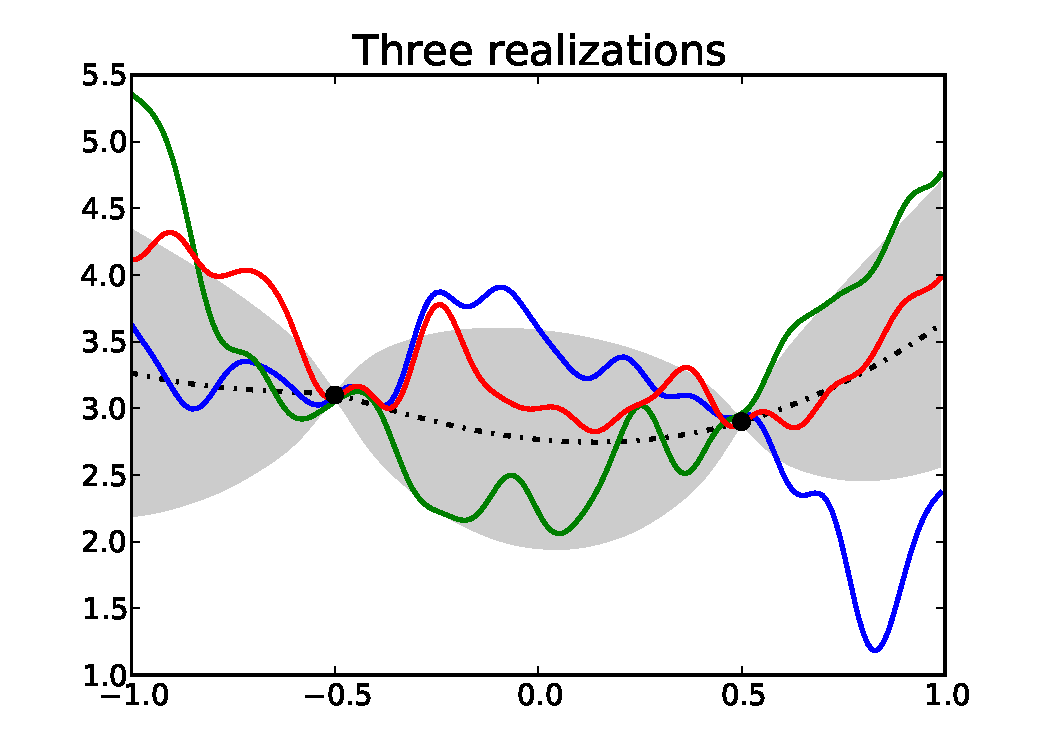
\epsfig{file=figs/basiscov.pdf,width=8cm}
        \caption{Three realizations of an observed Gaussian process whose covariance is an instance of \code{BasisCovariance}. The basis in this case is function \code{fourier_basis} from module \code{cov_funs}. 25 basis functions are used.}
    \label{fig:basiscov}
\end{figure}

It is possible to create random functions from linear combinations of finite sets of basis functions $\{e\}$ with random coefficients $\{c\}$:
\begin{eqnarray*}
    f(x) = M(x) + \sum_{i_0=0}^{n_0-1}\ldots \sum_{i_{N-1}=0}^{n_{N-1}-1} c_{i_1\ldots i_{N-1}} e_{i_1\ldots i_{N-1}}(x), \\
    \{c\}\sim \textup{N}(0,K).
\end{eqnarray*}
It follows that $f$ is a Gaussian process with mean $M$ and covariance defined by
\begin{eqnarray*}
    C(x,y)=\sum_{i_0=0}^{n_0-1}\ldots \sum_{i_{N-1}=0}^{n_{N-1}-1} \sum_{j_0=0}^{n_0-1}\ldots \sum_{j_{N-1}=0}^{n_{N-1}-1} e_{i_0\ldots i_{N-1}}(x) e_{j_0\ldots j_{N-1}}(x) K_{i_0\ldots i_{N-1}, j_0\ldots j_{N-1}},
\end{eqnarray*}
where $K$ is the covariance of the coefficients $c$.

Particularly successful applications of this general idea are:
\begin{description}
    \item[Random Fourier series:] $e_i(x) = \sin(i\pi x/L)$ or $\cos(i\pi x/L)$. See \cite{spanos}.
    \item[Gaussian process convolutions:] $e_i(x) = \exp(-(x-\mu_n)^2)$. See \cite{convolution}.
    \item[B-splines:] $e_i(x) = $ a polynomial times an interval indicator. See \href{http://en.wikipedia.org/wiki/Basis_B-spline}{Wikipedia}'s article.
\end{description}
Such representations can be very efficient when there are many observations in a low-dimensional space, but are relatively inflexible in that they generally produce realizations that are infinitely differentiable. In some applications, this tradeoff makes sense.

This package supports basis representations via the \code{BasisCovariance} class:
\begin{verbatim}
    C = BasisCovariance(basis, cov, **basis_params)
\end{verbatim}
The arguments are:
\begin{description}
    \item[\code{basis}:] Must be an array of functions, of any shape. Each basis function will be evaluated at $x$ with the extra parameters. The basis functions should obey the same calling conventions as mean functions: return values should have shape \code{x.shape[:-1]} unless $x$ is one-dimensional, in which case return values should be of the same shape as \code{x}. Note that each function should take the entire input array as an argument.
    \item[\code{cov}:] An array whose shape is either:
        \begin{itemize}
            \item Of the same shape as \code{basis}. In this case the coefficients are assumed independent, and \code{cov[i[0],...,i[N-1]]} (an $N$-dimensional index) simply gives the prior variance of the corresponding coefficient.
            \item Of shape \code{basis.shape * 2}, using \proglang{Python}'s convention for tuple multiplication. In this case \code{cov[i[0],...,i[N-1], j[0],...,j[N-1]]} (a $2N$-dimensional index) gives the covariance of $c_{i_0\ldots i_{N-1}}$ and $c_{j_1\ldots j_{N-1}}$.
        \end{itemize}
        Internally, the basis array is ravelled and this covariance tensor is reshaped into a matrix. This input convention makes it easier to keep track of which covariance value corresponds to which coefficients. The covariance tensor must be symmetric (\code{cov[i[0],...,i[N-1], j[0],...,j[N-1]]} $=$ \code{cov[j[0],...,j[N-1], i[0],...,i[N-1]]}), and positive semidefinite when reshaped to a matrix.
    \item[\code{basis_params}:] Any extra parameters required by the basis functions.
\end{description}

\section{Separable bases}

Many bases, such as Fourier series, can be decomposed into products of functions as follows:
\begin{eqnarray*}
    e_{i_0\ldots i_{N-1}}(x) = \prod_{j=0}^{N-1}e_{i_j}^j(x)
\end{eqnarray*}
Basis covariances constructed using such bases can be represented more efficiently using \code{SeparableBasisCovariance} objects. These objects are constructed just like \code{BasisCovariance} objects, but instead of an $n_0\times \ldots \times n_{N-1}$ array of basis functions they take a nested lists of functions as follows:
\begin{verbatim}
    basis = [ [e[0][0], ... ,e[0][n[0]-1]]
                       ...
              [e[N-1][0], ... ,e[N-1][n[N-1]-1]] ].
\end{verbatim}
For an $N$-dimensional Fourier basis, each of the \code{e}'s would be a sine or cosine; frequency would increase with the second index. As with \code{BasisCovariance}, each basis needs to take the entire input array \code{x} and \code{basis_params} as arguments. See \code{fourier_basis} in \code{examples/gp/basiscov.py} for an example.

\subsection{Example}

Once created, a \code{BasisCovariance} or \code{SeparableBasisCovariance} object behaves just like a \code{Covariance} object, but it and any \code{Mean} and \code{Realization} objects associated with it will take advantage of the efficient basis representation in their internal computations. An example of \code{SeparableBasisCovariance} usage is given in \code{pymc/examples/gp/basis_cov.py}. Compare its output in figure \ref{fig:basiscov} to that in figure \ref{fig:obs}.
